\chapter{Metodología}\label{ch:chapter_3}


\section{Programación extrema}

La Programación Extrema o \textit{extreme programming} (XP) es una metodología ágil de desarrollo de software que se
enfoca en mejorar la calidad del software y la capacidad de respuesta a las necesidades cambiantes del cliente.
Introducida por Kent Beck en el libro \textit{Extreme Programming Explained: Embrace Change}~\cite{book_beck_1999},
XP promueve la colaboración intensa entre los desarrolladores y los clientes, ciclos de
desarrollo cortos y frecuentes, y la entrega continua de pequeñas mejoras.

Una de las principales ventajas de XP es su capacidad para adaptarse rápidamente a los cambios en los requisitos del
cliente, lo que facilita que el producto final satisfaga las necesidades del negocio.


\section{Desarrollo dirigido por pruebas}

El desarrollo dirigido por pruebas o \textit{test driven development} (TDD) es una práctica de desarrollo de software.
Este enfoque fue popularizado por Kent Beck, uno de los pioneros de las metodologías ágiles, en su libro
\textit{Test Driven Development: By Example}~\cite{book_beck_2003}.
TDD se basa en ciclos cortos de desarrollo donde se escribe una prueba, se implementa el código necesario para pasar la
prueba y luego se reescribe el código para mejorar su estructura sin cambiar su comportamiento.


\section{Iterativo incremental}\label{sec:iterativo_incremental}

El enfoque iterativo incremental es una metodología utilizada en el desarrollo de software que combina dos modelos:
el iterativo y el incremental.
Esta metodología es popular en el desarrollo ágil y se centra en desarrollar un sistema a través de ciclos repetidos
(iteraciones) y en la construcción gradual de funcionalidad (incrementos).

El término ``iterativo'' se refiere a la repetición de un conjunto de actividades a lo largo del ciclo de vida del
desarrollo del software.
En cada iteración, se planea, desarrolla y evalúa una parte del sistema.

El término ``incremental'' se refiere a la construcción del sistema mediante adiciones sucesivas de componentes y
funcionalidades.
Cada incremento agrega una parte funcional del sistema hasta que el producto está completo.


\section{Gestión visual de procesos}

La gestión visual de procesos o \textbf{kanban} es un método de gestión de proyectos que se originó en la industria
manufacturera japonesa, específicamente en Toyota, como una forma de mejorar la eficiencia de la
producción~\cite{book_anderson_2010}.

El término significa ``tarjeta visual` en japonés, y el método se basa en el uso de tarjetas visuales para
representar tareas en un tablero, permitiendo a los equipos ver el estado del trabajo en progreso de un
vistazo.

\begin{figure}[ht]
    \begin{center}
        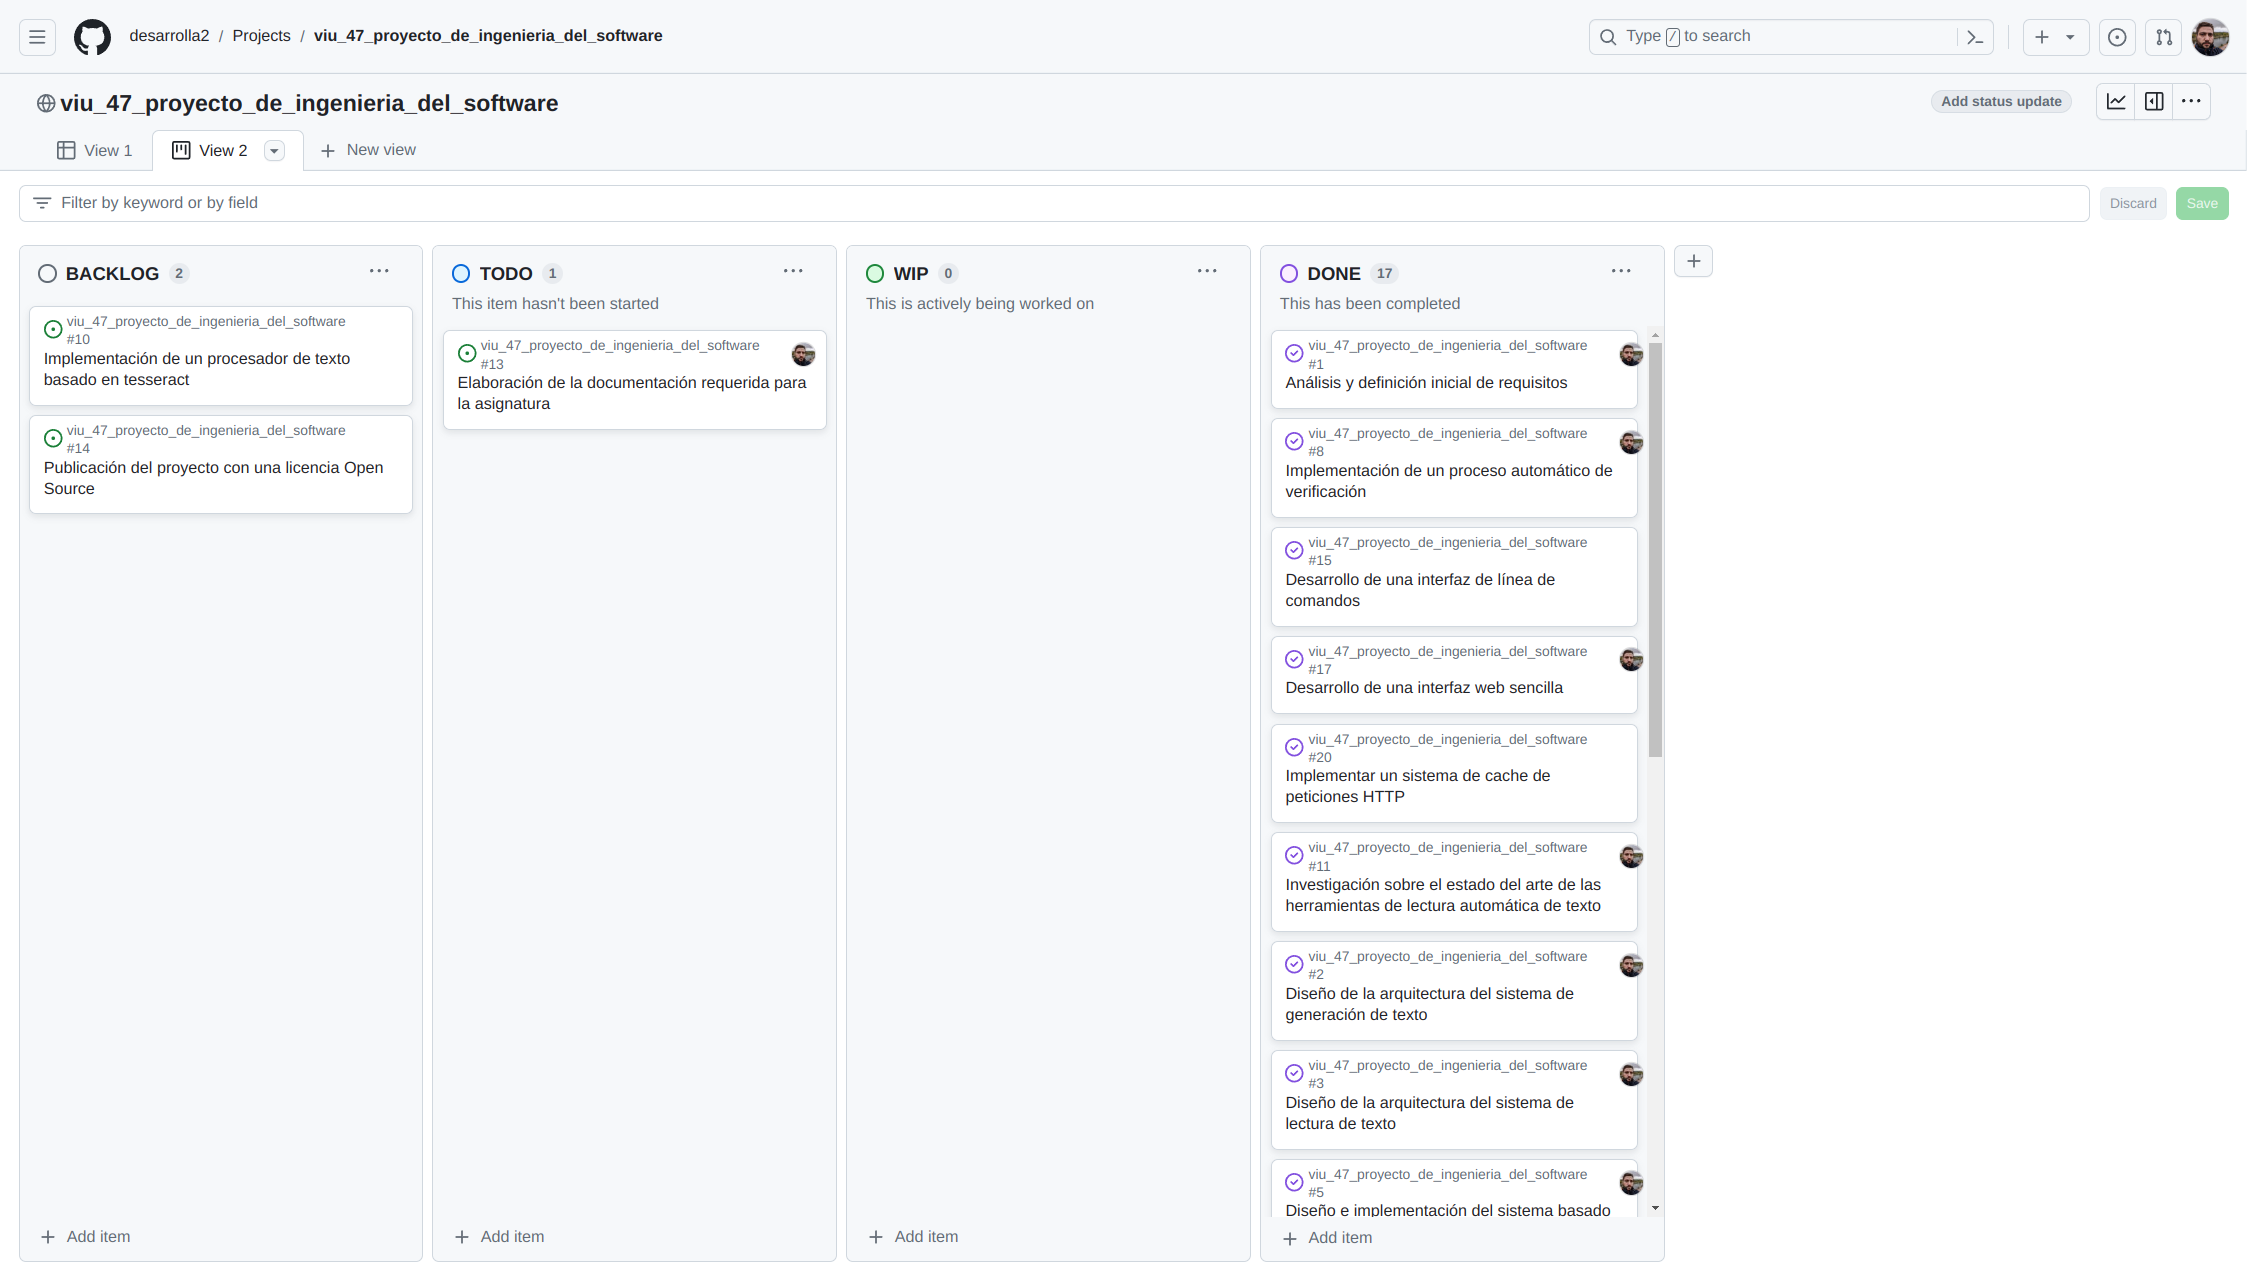
\includegraphics[width=\textwidth]{./chapter/3/images/chapter_3.kanban}
        \caption{Tablero kanban del proyecto}
        \label{fig:chapter_3.kanban}
    \end{center}
\end{figure}

Kanban promueve la mejora continua, la flexibilidad y la eficiencia, ayudando a los equipos a gestionar el flujo de
trabajo y a identificar cuellos de botella rápidamente.

En la figura~\ref{fig:chapter_3.kanban} aparece el tablero kanban utilizado en el desarrollo de este proyecto.


